\chapter{Modélisations de l'audiovisuel}\label{chap:mav}

\section{Cahier des charges fonctionnel}
% \addcontentsline{toc}{section}{Cahier des charges fonctionnel}
\e{
Qu'est-ce qu'un objet audiovisuel et particulier comment peut-on aborder le document audiovisuel ? (\ref{sec:dav})
Comment les produits de la chaîne audiovisuelle sont gérées par les systèmes informatiques, quelles opérations sont menées sur ces objets ? (\ref{sec:gest})
Comment décrit-on les objets audiovisuels, comment s'organisent la construction ou la récolte de ces informations dans la chaîne de production ? (\ref{sec:desc})
}


\subsection{Scénario de réutilisation multiple}\label{sec:ex-reuse}
Pour bien saisir la finesse des différentes opérations possibles, nous proposons de prendre un exemple.
Imaginons une chaîne de télévision qui souhaite réaliser la captation d'un évènement culturel (par exemple un opéra, une pièce de théâtre, un concert etc.). 
Les producteurs de la chaîne sont intéressés par trois types de contenus qui seront ensuite exploités de quatre manières différentes (voir Figure \ref{img:intro:reuse}):
\begin{listenum}
	\item[a.] la \e{captation de l'évènement} en tant que tel.
	\item[b.] des \e{entrevues avec l'équipe} (metteur en scène, talents sur scène, programmateur etc.). 
	\item[c.] des \e{commentaires du public} avant ou après l'évènement.\\

	\item une partie de tous les types de contenu sera utilisée pour construire un sujet destiné à un \e{journal télévisé}. 
	\item un montage raccourci de l'évènement et des commentaires du public seront utilisés pour produire une \e{bande-annonce diffusée sur le Web}.
	\item un montage de la captation de l'évènement, des bonus comprenant les entrevues avec l'équipe ainsi que la bande-annonce utilisant les commentaires spectateurs seront intégrés dans le \e{DVD}.	 
	\item tout ou partie du contenu filmé pourra être transmis ou vendu à des \e{organisations tierces}. 
\end{listenum}

\begin{figure}[ht!]
\centering
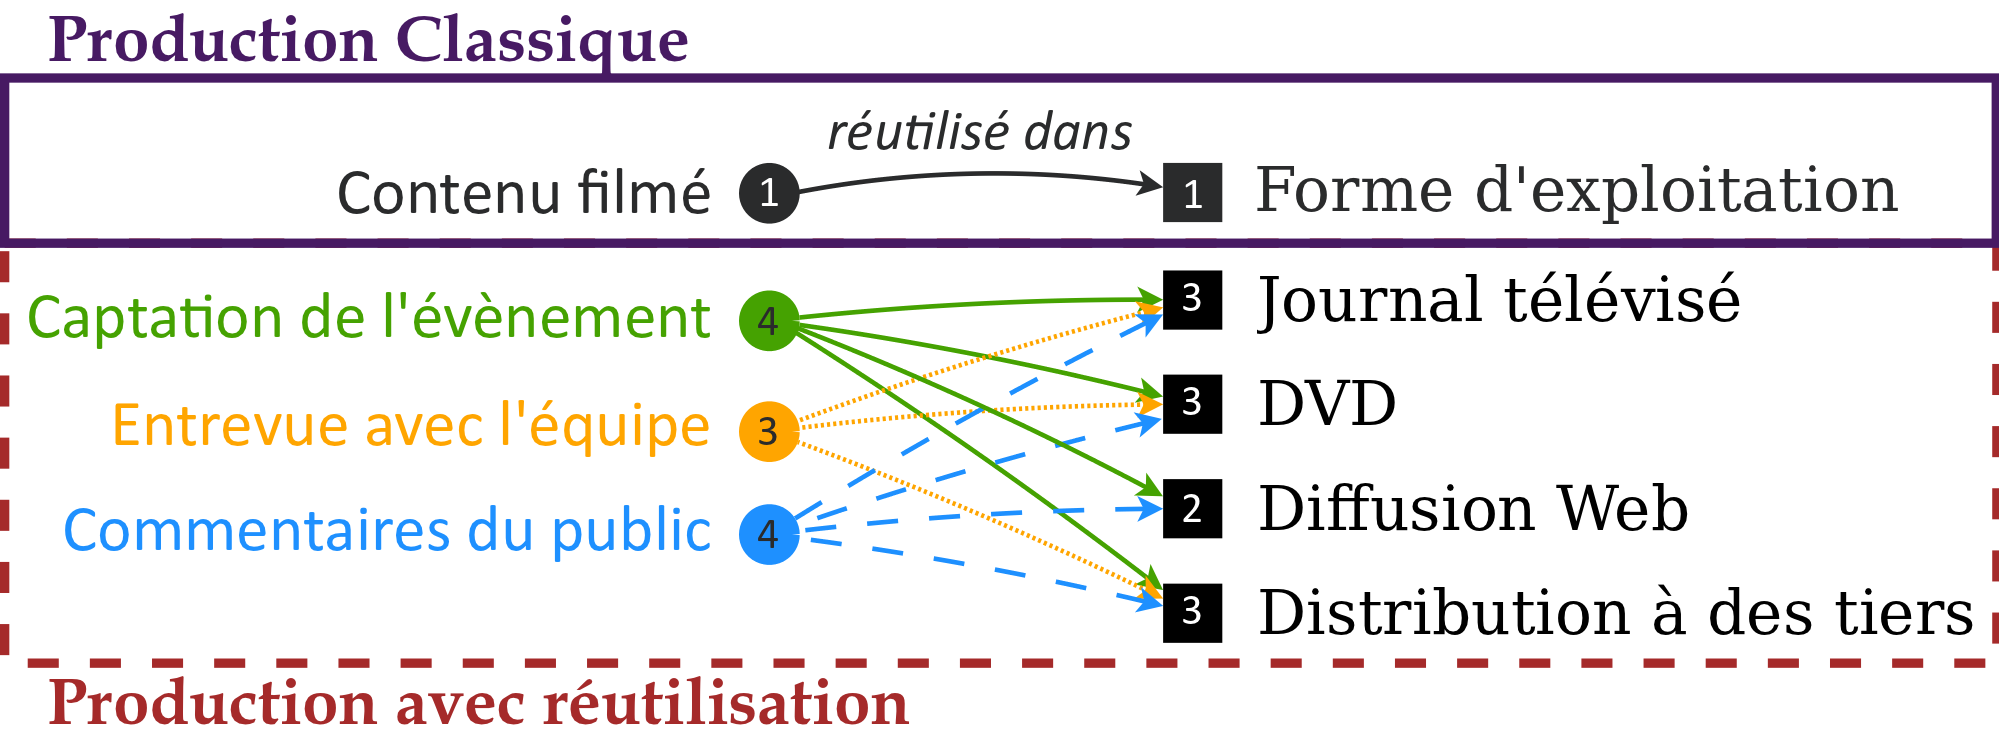
\includegraphics[width=0.7\textwidth]{images/UC-Tahnhauser-v1fr.png}
\caption{Modèle de la production classique comparé avec une production avec réutilisation}
\label{img:intro:reuse}
\end{figure}

Chaque cas de réutilisation tire sa matière première d'à peu près la même base de contenu filmé, mais en tire partie d'une manière propre à chaque forme d'exploitation visée. 
En effet, chaque audience a ses attentes, de même qu'il existe des contraintes techniques spécifiques pour chaque contexte d'exploitation. 
%En effet, il existe des contraintes techniques et des attentes spécifiques à chaque contexte d'exploitation. 

Ces spécificités exigent des variations dans la qualité de l'encodage, le format d'encapsulation utilisé, le montage réalisé, l'habillage du contenu etc. 
Par exemple, les contraintes de diffusion sur le Web implique d'encoder la vidéo dans un format spécifique et de multiples résolutions, généralement plus petites que pour la diffusion télévisée. 
Ensuite, le montage d'une bande-annonce possède un rythme généralement plus rapide que celui des bonus de DVD. 
Finalement, les cas d'exploitation gérés par la chaîne de télévision posséderont un habillage spécifique (logo de la chaîne, message d'annonces etc.) que ne partageront pas forcément les versions vendu à des organisations tierces. 

L'exemple des commentaires du public -- voir la Figure \ref{img:intro:reuse-process} -- permet de montrer à quels moments des transformations doivent être effectuées afin de produire les différentes formes d'exploitation :
\begin{liste} 
	\item[$\bullet$] On considère que deux commentaires de spectateur ont été tournés. 
	\item[$\bullet$] Un des commentaires est intégré au montage du journal télévisé, alors que les deux sont utilisés pour créer la bande-annonce. La bande-annonce est elle-même intégrée au montage du DVD. 
	\item[$\bullet$] Au moment de la finition, l'encodage de la bande-annonce est adapté à la qualité DVD et Web. De même, le journal télévisé est encodé à la fois pour une diffusion en définition standard (SD) et haute-définition (HD).
\end{liste}


\begin{figure}[ht!]
\centering
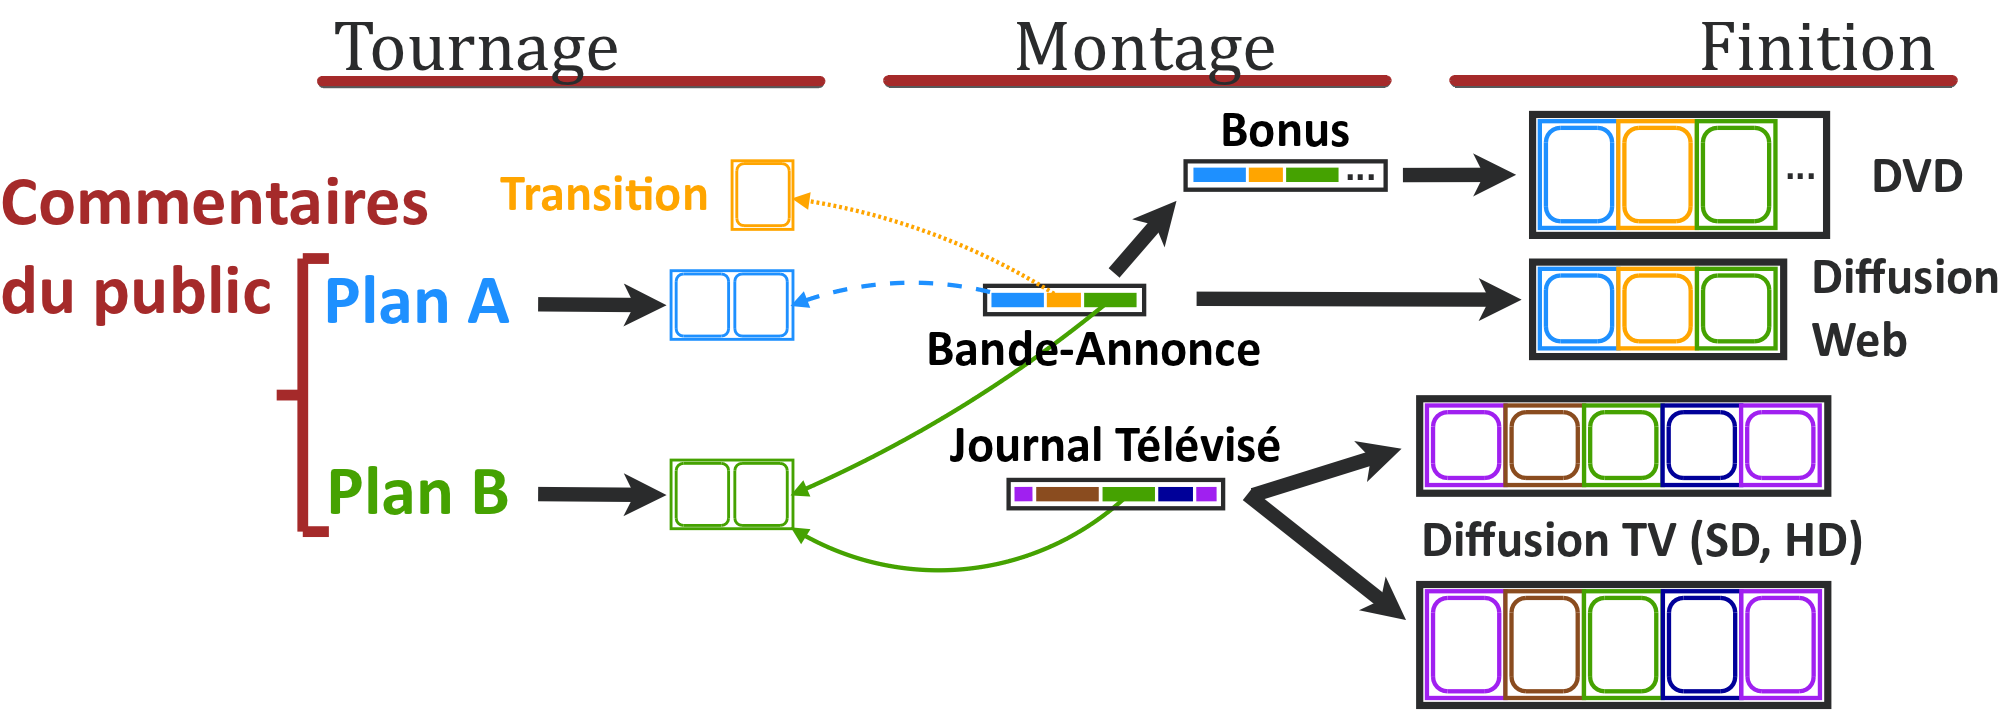
\includegraphics[width=0.8\textwidth]{images/EX-Content-Production-v7fr.png}
\caption{Étapes et transformations des contenus pour chaque forme d'exploitation des commentaires des spectateurs}
\label{img:intro:reuse-process}
\end{figure}

Dans cet exemple, on distingue deux types d'opérations effectuées sur le contenu ; 
la sélection de séquences au moment du montage qui correspond à une décision éditoriale (quel contenu va-t-on présenter à l'audience ?) ; 
la tranformation de l'enregistrement du contenu qui correspond à des choix techniques (quelle méthode d'enregistrement va-t-on utiliser ?).
Afin de préciser la nature de ces opérations, nous présentons différentes approches de la réutilisation des contenus.



\section{Qu'est-ce qu'un objet audiovisuel ?}\label{sec:dav}
Quelles sont les manières de représenter les objets/contenus/documents audiovisuels, quelle sont les différences entre ces notions.

\cite{Morizet-mahoudeaux2005a} ; Définition de Media Asset etc. de l'Encyclopedia of Multimedia.